%%%%%%%%%%%%%%%%%%%%%%%%%%%%%section Boundary Conditions%%%%%%%%%%%%%%%%%%%%%%%%%%%%%%%%%%%%%%%%%%%%%%%%%%%%%%%%%%%%
%%%%%%%%%%%%%%%%%%%%%%%%%%%%%%%%%%%%%%%%%%%%%%%%%%%%%%%%%%%%%%%%%%%%%%%%%%%%%%%%%%%%%%%%%%%%%%%%%%%%%%%%%%%%%%%%%%
\section{Boundary Conditions}\label{sec:BC}
%%%%%%%%%%%%%%%%%%%%%%%%%%%%%%%%%%%% subsection General introduction to boundary conditions %%%%%%%%%%%%%%%%%%%%%%%%%%%%%%%%%%%%%%%%%%%%%%%%%%%%%%%%%%%%%%%%%%%%%
    \subsection{General introduction to boundary conditions}\label{subsec:General introduction to BC}
    \subsubsection{Equations of boundary conditions}\label{subsubsec:Equations of BC}
	  Boundary conditions (BC) are necessary for solving the  Maxwell's equations by using FDTD. They can limit the computation in a finite space but attaining the same solution just as in  infinite space.  \\
	  The following equations are the general boundary conditions at  arbitrary interface between two medium. There can be  charges (denoted as charge density $\rho_s$) or  currents (denoted as surface electric current density $\vec{\mathbf{J}}_s$ and  surface magnetic current density $\vec{\mathbf{M}}_s$) at the interface:
	  %%%%% BC EQ
	      \begin{eqnarray}
		  \hat{n}\cdot(\vec{\mathbf{D}}_2-\vec{\mathbf{D}}_1) &=&\rho_s  \\
		  \hat{n}\cdot(\vec{\mathbf{B}}_2-\vec{\mathbf{B}}_1) &=&0  \\
		  \hat{n}\times(\vec{\mathbf{E}}_2-\vec{\mathbf{E}}_1) &=&-\vec{\mathbf{M}}_s \\
		  \hat{n}\times(\vec{\mathbf{H}}_2-\vec{\mathbf{H}}_1) &=&\vec{\mathbf{J}}_s
		  \label{eq:General boundary conditions}
	      \end{eqnarray}

    \subsubsection{Four  types of boundary conditions in OpenEMS}\label{subsubsec:Four particularly usefull BC}
	Under some special given conditions or assumptions, the boundary conditions(\ref{eq:General boundary conditions}) have  respective forms and they are convenient for the most simulations. These BC are called as:
       \begin{myindentpar}[2cm]
	       perfect electric conductor (\textbf{PEC}), \\
	     perfect magnetic conductor (\textbf{PMC}),\\
	      \textbf{MUR} absorbing boundary condition,\\
              perfectly matched layer (\textbf{PML}) absorbing boundary condition.
       \end{myindentpar}
The types of these BC are stored in \matv{BoundaryCond}, a field of the structure  \matv{FDTD} in MATLAB. \phantomsection \label{para:BoundaryCond}
    \subsection{Setting boundary conditions}\label{subsec:Setting boundary conditions in OpenEMS with function SetBoundaryCond}
%%%%%%%%%%%%%%%%%%%%%%% FUNCTION  InitFDTD %%%%%%%%%%%%%%%%%%%%%%%%%%%%%%%%%%%5
\begin{FontNameFunct}{SetBoundaryCond()}
\phantomsection \label{func:SetBoundaryCond}
\end{FontNameFunct}

%%%%%%%%%%%%%%%%%%%%%%%%%%%% Purpose
\begin{FontDescr}{Purpose:}
Set  boundary conditions of Maxwell's equations for simulation.% Assign the field \matv{BoundaryCond} of structure \matv{FDTD}  in MATLAB.
\end{FontDescr}

%%%%%%%%%%%%%%%%%%%%%%%%%%%% Syntax
\begin{FontDescr}{Syntax:}
      \begin{lstlisting}
FDTD = SetBoundaryCond(FDTD, BC, varargin)
      \end{lstlisting}
\end{FontDescr}

\begin{FontDescr}{Description:}
%%%%%%%%%%%%%%%%%%%%%%%%%%%% BC
    \begin{FontPara}{BC} \phantomsection \label{para:BC}
   \matv{BC} provides the types of the boundary conditions to the 6 boundaries in the 3D simulating space.
          \matv{BC} is defined either as a \textbf{vector} or as a \textbf{cell} with 6  elements in MATLAB. \vspace{2mm}\\
          If  \matv[para:T_xmin]{T\_xmin}\phantomsection \label{para:T_xmin},
	  \matv[para:T_xmax]{T\_xmax}\phantomsection \label{para:T_xmax},
	  \matv[para:T_ymin]{T\_ymin}\phantomsection \label{para:T_ymin},
	  \matv[para:T_ymax]{T\_ymax}\phantomsection \label{para:T_ymax},
	  \matv[para:T_zmin]{T\_zmin}\phantomsection \label{para:T_zmin} and
	  \matv[para:T_zmax]{T\_zmax}\phantomsection \label{para:T_zmax} are  arguments which denote for the types of the conditions at the respective boundaries, then \matv{BC} can be defined as a vector or a cell as following.\vspace{2mm}\\
    \begin{itemize}
       %%%%%%%%%%%% vector BC
        \item  \matv{BC} is defined as a \textbf{vector}
	\begin{myindentpar}
% 	  \lstset{caption={\matv{BC} in the form of a vector},label=BCinvector}
	  \begin{lstlisting}[caption={\matv{BC} in the form of a vector},label=BCinvector]
 BC=[T_xmin T_xmax T_ymin T_ymax T_zmin T_zmax];
	  \end{lstlisting}
          Each  element (\matv[para:T_xmax]{T\_*min} or\matv[para:T_xmax]{T\_*max}) of the vector  must be  one of the following numbers
	    \begin{myindentpar}
	      \matval{0}   \qquad  (for PEC)\\
	      \matval{1}   \qquad  (for PMC)\\
	      \matval{2}   \qquad  (for MUR)\\
	      \matval{3}   \qquad  (for PML with 8 default layers).
	    \end{myindentpar}
      \end{myindentpar}
          %%%%%%%%%%%% Cell BC
          \item   \matv{BC} is defined as a \textbf{cell}
	  \begin{myindentpar}
% 	   \lstset{caption={\matv{BC} in the form of a cell},label=BCincell}
	  \begin{lstlisting}[caption={\matv{BC} in the form of a cell},label=BCincell]
 BC={T_xmin T_xmax T_ymin T_ymax T_zmin T_zmax};
	  \end{lstlisting}
	  of which   each  element(\matv[para:T_xmax]{T\_*min} or\matv[para:T_xmax]{T\_*max})  must be set as one of the following strings
	  \begin{myindentpar}
	     \matval{PEC} \qquad   (for PEC)\\
	     \matval{PMC} \qquad   (for PMC)\\
	     \matval{MUR}  \qquad  (for MUR)\\
	     \matval{PML\_x} \qquad   (for PML. \texttt{x} is  the PML size. It should be replaced with an integer in an interval from 4 to 50).
	  \end{myindentpar}
	\end{myindentpar}
\end{itemize}
	  So the element \texttt{BC}($i$) or \texttt{BC}\{$i$\} represents for the type of the  condition at the respective boundary as showed in the following table
	  \begin{table}[htb]\centering
	  \begin{tabular}{l|l}
	  \texttt{BC($i$)} or \texttt{BC\{$i$\}} & Respective position of the boundary\\ \hline
		 \texttt{BC(1)} or  \texttt{BC\{1\}} & where x or $\rho$ is minimum\\
		 \texttt{BC(2)} or  \texttt{BC\{2\}}& where x or $\rho$ is maximum\\
		 \texttt{BC(3)} or  \texttt{BC\{3\}}& where y or $\varphi$ is minimum\\
		 \texttt{BC(4)} or  \texttt{BC\{4\}}& where y or $\varphi$is maximum\\
		 \texttt{BC(5)} or  \texttt{BC\{5\}}& where z is minimum\\
		 \texttt{BC(6)} or  \texttt{BC\{6\}}& where z is maximum.
	  \label{Elements of BC and the rescpective boundaries}
	  \end{tabular}\caption{Mapping relationship between the elements of \matv{BC} and the  boundaries.}
	  \end{table}
	  
            %%%%%%%%%%%%%%%% Info
	\info{In a cylindrical system,  the elements of \matv{BC} represent for the types of boundary conditions at $\rho$, $\varphi$, $z$ instead of at $x, y, z$ (see listing \ref{ListingCylinBC}). If there are no  BC at $\rho\_min=0$ or at $\varphi$,   the elements of  \matv{BC} for the  corresponding boundaries conditions   can be set as \matval{0} or \matval{PEC} just in a virtual form for computation(see listing \ref{listing:SettingofBC in a cylin.}). For these cases, the corresponding elements have nothing to do with the boundaries conditions indeed.} \\
	  \lstset{caption={\matv{BC} in  cylindrical coordinate system},label={ListingCylinBC}}
         \begin{lstlisting}
% as a vector
  BC=[T_rhomin T_rhomax T_phimin T_phimax T_zmin T_zmax];
% as a cell
  BC={T_rhomin T_rhomax T_phimin T_phimax T_zmin T_zmax}
	  \end{lstlisting}%%question: phi_min and phi_max don't form a closed circle,then???
    \end{FontPara}
\end{FontDescr}

\begin{FontDescr}{Optional Arguments:}
			%%%%%%%%%%%%%% MUR_PhaseVelocity
    \begin{FontPara}[para:MUR_PhaseVelocity]{MUR\_PhaseVelocity} \phantomsection \label{para:MUR_PhaseVelocity}
	It defines a phase-velocity and  it's used by the MUR-abc. It's useful e.g. for dispersive waveguides.
    \end{FontPara}
			%%%%%%%%%%%%%% PML_Grading
    \begin{FontPara}[para:PML_Grading]{PML\_Grading} \phantomsection \label{para:PML_Grading}
	Or \matv[para:PML_Grading]{gradFunction}. It defines the PML grading function.\vspace{2mm}
			    Predefined variables in this grading function are:
			      \begin{myindentpar}
				\matval{D}  = depth in the PML in meter\\
				\matval{dl} = mesh delta inside the PML in meter\\
				\matval{W}  = width (length) of the PML in meter\\
				\matval{N}  = number of cells for the PML\\
				\matval{Z}  = wave impedance at the current depth and position
			    \end{myindentpar}
    \end{FontPara}
\end{FontDescr}

%%%%%%%%%%%%%%%%%%%%% Examples.
	\begin{FontDescr}{Examples:}
	  \begin{itemize}
	  %%%%%%%1st step
	  \item    Setting boundary conditions in a Cartesian coordinate system.\\
		1st step: \matv{BC} assignment
	      \begin{myindentpar}
		    \begin{lstlisting}[caption={\matv{BC} assignment as fig \ref{fig:Ex. 1st of SetBoundaryCond} },label={listing:1st SettingofBC}]
		    %using numbers
		    BC=[ 1     1     0     0     2     3     ]
		    %or using equivalent strings
		    BC={'PMC' 'PMC' 'PEC' 'PEC' 'MUR' 'PML_8'}
				\end{lstlisting}
		    Both above vector and cell set  the x-boundaries (perpendicular to $x$ axis) as PMC, and the y-boundaries (perpendicular to $y$ axis) as PEC, the zmin-boundary (perpendicular to $z$ axis and $z$ is minimum) as MUR but the zmax-boundary (perpendicular to $z$ axis and $z$ is maximum) as PML with 8 layers. These boundary conditions are showed in fig \ref{fig:Ex. 1st of SetBoundaryCond}.
			\begin{figure}[ht]
				\centering
			      \subfloat[\matv{BC} at $x$ and $y$]{\includegraphics[width=0.4\textwidth]{svg/BCXY1.eps}}\qquad
			      \subfloat[\matv{BC} at $x$ and $z$]{\includegraphics[width=0.4\textwidth]{svg/BCXZ1.eps}}\qquad
	  %\includegraphics[width=0.9\textwidth]{svg/BCXY.eps}
				\caption[1st example for the setting of boundary conditions]{\matv{BC} \texttt{=[1 1  0 0  2 3]} , see listing \ref{listing:1st SettingofBC}}
				\label{fig:Ex. 1st of SetBoundaryCond}
			  \end{figure}
	      \end{myindentpar}
	  %%%%%%%2nd step
		2nd step: Updating the \matv{FDTD} structure with \matv{BC} or other andvanced arguments.
		\begin{myindentpar}
			      \begin{lstlisting}
	    % without advanced arguments
	    FDTD=SetBoundaryCond(FDTD,BC);
			      \end{lstlisting}
				or
			      \begin{lstlisting}
	    % with advanced argument for MUR
	    FDTD=SetBoundaryCond(FDTD,BC,...
		'MUR_PhaseVelocity',300000000);
				  \end{lstlisting}
			      \begin{lstlisting}
	    % with advanced argument for PML
	    FDTD=SetBoundaryCond(FDTD,BC,...
		'PML_Grading','-log(1e-6)*log(2.5)/...
		(2*dl*pow(2.5,W/dl)-1)*pow(2.5, D/dl)/Z');
			      \end{lstlisting}
	      \end{myindentpar}
	  %%%%%%%%%% cylindrical sys
	  \item Setting boundary conditions in a cylindrical coordinate system.\\
	  If there are no boundaries at  $\rho_{min}=0$ and at any $\varphi$, then please set the elements as \matval{0} or \matval{PEC} as the following example.
	      \begin{lstlisting}[caption={\matv{BC} assignment in a cylindrical coordinate system as fig \ref{fig:Ex. SetBoundaryCond in cylin.}},label={listing:SettingofBC in a cylin.}]
		  % no boundaries at rhomin=0 , phi_min and phi_max
		  BC=[0 1 0 0 3 3];
		  %or using equivalent strings
		  BC={'PEC' 'PMC' 'PEC' 'PEC' 'PML_8' 'PML_8'}
		  FDTD=SetBoundaryCond(FDTD,BC);
				  \end{lstlisting}
	      \begin{figure}[ht]
				    \centering
				  \includegraphics[width=0.6\textwidth]{svg/CylinBCXY.eps}\qquad
				    \caption[ Setting virtual boundary conditions ($\rho_{min}=0$, $\varphi_{min}=-\pi$ and   $\varphi_{max}=\pi$) in a cylindrical coordinate system]{Virtual boundary conditions (at $\rho_{min}=0$, $\varphi_{min}=-\pi$ and   $\varphi_{max}=\pi$)  in a cylindrical coordinate system. See listing \ref{listing:SettingofBC in a cylin.}}
				    \label{fig:Ex. SetBoundaryCond in cylin.}
			      \end{figure}
	  %%%%%%%%%%%%% half cylindrical
	  \item If there are boundaries at $\rho_{min}\neq0$ and $\varphi$, then please set the elements as corresponding number or string.
	  \begin{lstlisting}[caption={\matv{BC} assignment in a cylindrical coordinate system as fig \ref{fig:Ex. SetBoundaryCond in cylin. Half}},label={listing:SettingofBC in a cylin. Half}]
		  % no boundaries at rhomin=0 , phi_min and phi_max
		  BC=[0 1 0 1 0 3];
		  %or using equivalent strings
		  BC={'PEC' 'PMC' 'PEC' 'PMC' 'PEC' 'PML_8'}
		  FDTD=SetBoundaryCond(FDTD,BC);
				  \end{lstlisting}
	      \begin{figure}[H]
				    \centering
	  \subfloat[Boundaries conditions at $z$  ]{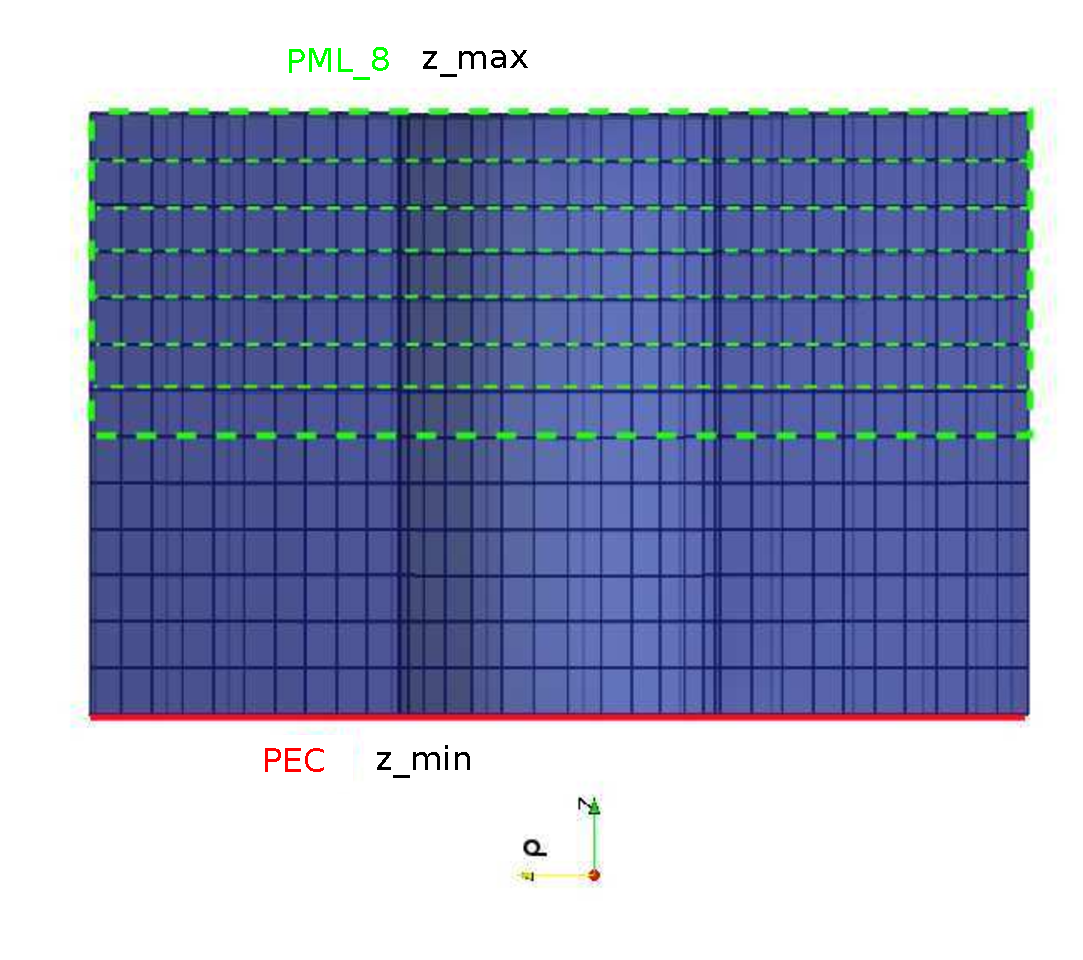
\includegraphics[width=0.6\textwidth]{svg/CylinBCXZ2.eps}}\qquad
	  \subfloat[ Boundaries conditions at $\rho$ and $\varphi$ ]{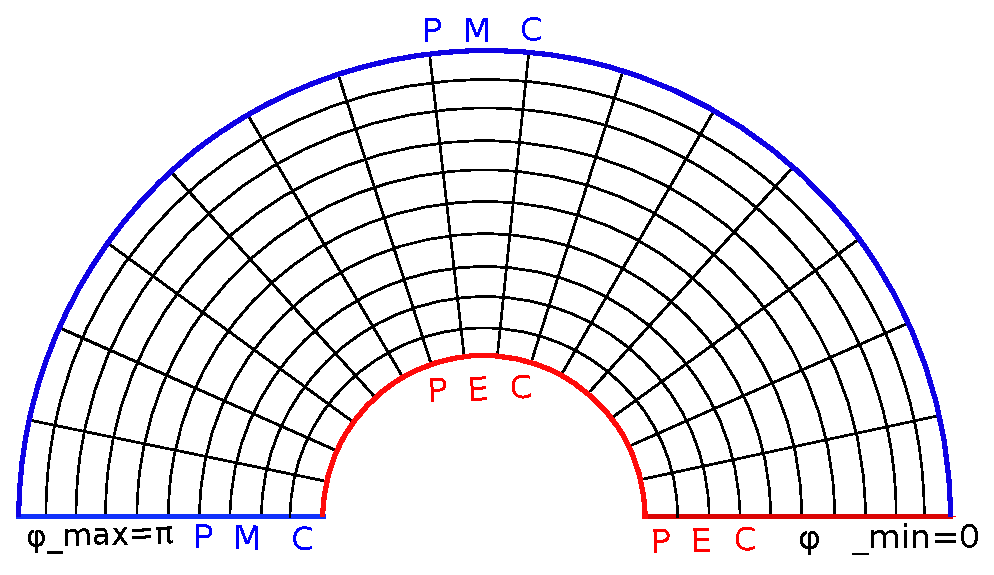
\includegraphics[width=0.55\textwidth]{svg/CylinBCXY2.eps}}\qquad
				    \caption[ Setting  boundary conditions in a cylindrical coordinate system]{An example of boundary conditions in a cylindrical coordinate system. See listing \ref{listing:SettingofBC in a cylin. Half}}
				    \label{fig:Ex. SetBoundaryCond in cylin. Half}
			      \end{figure}
	  \end{itemize}
	\end{FontDescr}
 \warning{Avoid to place any excitation in the  PML.}
